%
%   Chapter Method
%
%   Qing-Cheng Li (r01922024 at csie dot ntu dot edu dot tw)
%   R.O.C.103.07
%
\chapter{研究方法}
\label{c:method}

本研究擬自內容串流中偵測實體的特性,
而實體的特性之一:實體間關係,則可以語句樣式表現,
因此本研究主要利用語句樣式來偵測這樣的特性是否存在。
本章將介紹所使用的資源、
樣式比對、樣式篩選、與特性歧義的問題與解決方法。

\section{以樣式偵測特性}
當我們在字裡行間要描述一個實體的特性時,
應該會有某些特定的樣式。
例如我們知道Jobs的出生地這個特性是San Francisco,
我們可能會以「Jobs was born in San Francisco」這樣的句子來表達這個概念。
而在上述句子之中「was born in」就是一個可以用來表示出生地此一實體特性的樣式,
當我們在句子中看到「was born in」時,就可以推測這個句子存在某人的出生地是某地這樣的實體特性。

基於這樣的想法,本研究將利用樣式的出現有無來決定是否存在實體特性,
設計了如圖\ref{i:process-v1} 的偵測流程。

圖\ref{i:process-v1} 中,首先要先有一份實體特性與樣式的關聯表,
知道每個實體特徵可以由哪些樣式來表達。
以上述例子來說,就會有一張表如表\ref{t:ext} 列有「出生地」這項實體特性,
並列出所有可以用來描述這項實體特性的樣式如「was born in 」、「[[adj]] childhood in」、「lived in」等;
表上也會有其他的實體特性如「生活地」,並列出樣式如「lived in」、「been working in」等可以描述這項實體特性。

\begin{table}
    \caption{實體特性與樣式範例關聯表}
    \label{t:ext}
    \begin{center}
    \footnotesize
    \begin{tabular}{|l|l|}
        \hline
        Property & Patterns \\
        \hline
        \multirow{3}{*}{出生地} & was bron in, \\
         & [[adj]] childhood in, \\
         & lived in\\
        \hline
        \multirow{2}{*}{生活地} & lived in, \\
         & been working in\\
        \hline
    \end{tabular}
    \end{center}
\end{table}

利用這份關係表,對文章中的句子進行比對,檢查關係表中的樣式是否出現。
若有出現,則這篇文章可能包含樣式對映的實體特性。
例如句子「Jobs was born in San Francisco」包含了「was bron in」,
但不包含「lived in」等其他樣式。
透過樣式「was born in」可以從關聯表中查到此樣式屬於實體特性「出生地」,
因此推論這個句子包含了「出生地」這項實體特性資訊。
樣式比對的細節會在第\ref{s:pattern-match} 節中詳述。

\begin{figure}
    \centering
    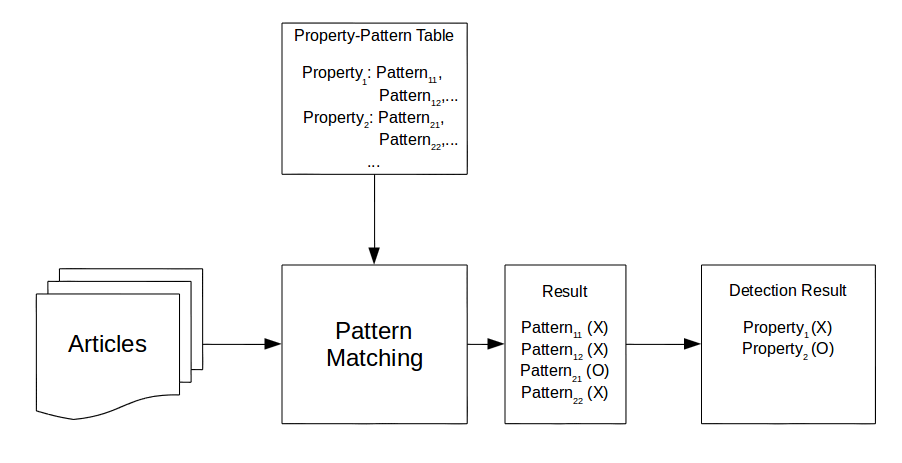
\includegraphics[width=0.9\textwidth]{images/03-process-v1}
    \caption{以樣式偵測特性流程概念}
    \label{i:process-v1}
\end{figure}

本研究擬利用PATTY已經提供的關係釋義表,
作為偵測流程中所需要的實體特性與樣式關聯表。
表中包含了知識庫YAGO內定義的實體間關係、
YAGO關係的領域與範圍(表\ref{t:yago-relation}),
以及可以用來描述這個關係的樣式。

%t:yago-relation
\begin{table}[t]
    \begin{center}
        \footnotesize
        \begin{tabular}{|l||c|c|c|}
        \hline
        YAGO Relation & Domain & Range & Number of patterns \\
        \hline
        actedIn & wordnet\_actor & wordnet\_movie & 2023 \\
        created & yagoLegalActor & Thing & 3215 \\
        dealsWith & wordnet\_location & wordnet\_location & 366 \\
        diedIn & wordnet\_person & wordnet\_city & 1352 \\
        directed & wordnet\_person & wordnet\_movie & 1228 \\
        graduatedFrom & wordnet\_person & wordnet\_university & 2129 \\
        happenedIn & wordnet\_event & yagoGeoEntity & 47 \\
        hasAcademicAdvisor & wordnet\_person & wordnet\_person & 632 \\
        hasCapital & wordnet\_location & wordnet\_location & 24 \\
        hasChild & wordnet\_person & wordnet\_person & 3620 \\
        hasWonPrize & yagoLegalActorGeo & wordnet\_award & 78 \\
        holdsPoliticalPosition & wordnet\_person & wordnet\_person & 1173 \\
        influences & wordnet\_person & wordnet\_person & 2461 \\
        isCitizenOf & wordnet\_person & wordnet\_country & 813 \\
        isKnownFor & yagoLegalActor & Thing & 1574 \\
        isLeaderOf & wordnet\_person & yagoLegalActorGeo & 465 \\
        isLocatedIn & yagoPermanentlyLocatedEntity & yagoGeoEntity & 1300 \\
        isMarriedTo & wordnet\_person & wordnet\_person & 4276 \\
        isPoliticianOf & wordnet\_person & wiki\_states\_of\_US & 465 \\
        livesIn & wordnet\_person & wordnet\_location & 718 \\
        participatedIn & yagoLegalActorGeo & Thing & 89 \\
        playsFor & wordnet\_person & wordnet\_organization & 1491 \\
        wasBornIn & wordnet\_person & wordnet\_city & 1226 \\
        worksAt & wordnet\_person & wordnet\_organization & 1602 \\
        \hline
        \end{tabular}
        \caption{YAGO Relations in PATTY}
        \label{t:yago-relation}
    \end{center}
\end{table}


光是這樣的流程並不足以偵測實體特性。
使用樣式來偵測實體特性還會有樣式覆蓋度(Coverage)、
品質(Quality)、可信賴度(Reliability)、與歧義性(Ambiguity)的問題。

樣式覆蓋度問題是指對於某個實體的特性,
在關係表內屬於這個實體特性的樣式佔所有可以表達該特性的樣式之比例。
以表\ref{t:ext} 為例,其中「生活地」這項實體特性表中列了2個樣式,
但實際上有更多的樣式可以表達這個概念,例如「been lived at」就沒有列在表中,
這樣有此樣式的句子就沒辦法被偵測為含有實體特性的句子。

樣式的品質則是一個字串到底能不能夠作為一個樣式,   
一個樣式的品質不高,那麼這樣的樣式有可能太廣泛的出現在句子之中,
致使這樣的樣式沒有辦法區辨出實體屬性。
例如PATTY關係釋義中的YAGO:actedIn內的樣式「links」就只有這一個單字,
用以描述實體特性顯得太廣泛了些,
以此擷取回的文章有包含實體特性的比例就較低。

樣式可信賴度則是一個樣式到底能不能用來表達實體特性。
例如,對於特性YAGO:diedIn,以「since worked in」來描述完全文不對題,
又如YAGO:wasBornIn中的樣式「also opened in」也無法描述特性。

而為了處理樣式的品質、可信賴度問題,
應該要在圖\ref{i:process-v1} 流程中的關聯表與樣式比對中增加一個樣式篩選的步驟,
篩選出可信賴、有一定品質的樣式來進行樣式比對,
此部份將於第\ref{s:select-pattern} 小節說明詳細內容。

經過樣式比對後,每篇文章可能存在數個樣式,
如果在關聯表中每個樣式只對映到一個關係,
那便沒有歧義。
但一個樣式可能存在於多個實體特性的關聯表內,
例如樣式「first met with」就被PATTY認為可以表示5種特性(hasAcademicAdvisor、isKnownFor、isMarriedTo、influences、hasChild)。
因此在樣式被比對出來之後,整個偵測流程中還需要一個消歧義的步驟,
決定當此樣式出現時,到底是5種特性中的哪一種?哪幾種?或者都沒有?
這個部份將在第\ref{s:pattern-disambiguity} 節中說明。

補上了樣式篩選與消歧義後的流程圖應修正為圖\ref{i:process-v2}。
樣式比對使用經過篩選的樣式,
比對出來後進行消歧義才完成偵測實體特性之流程。
由於偵測實體特性的流程對於每一分文件都是相同,且彼此互相獨立,
因此可以平行處理文件,如圖\ref{i:process-parallel} 所示,
處理內容串流的大量文件。

\begin{figure}
    \centering
    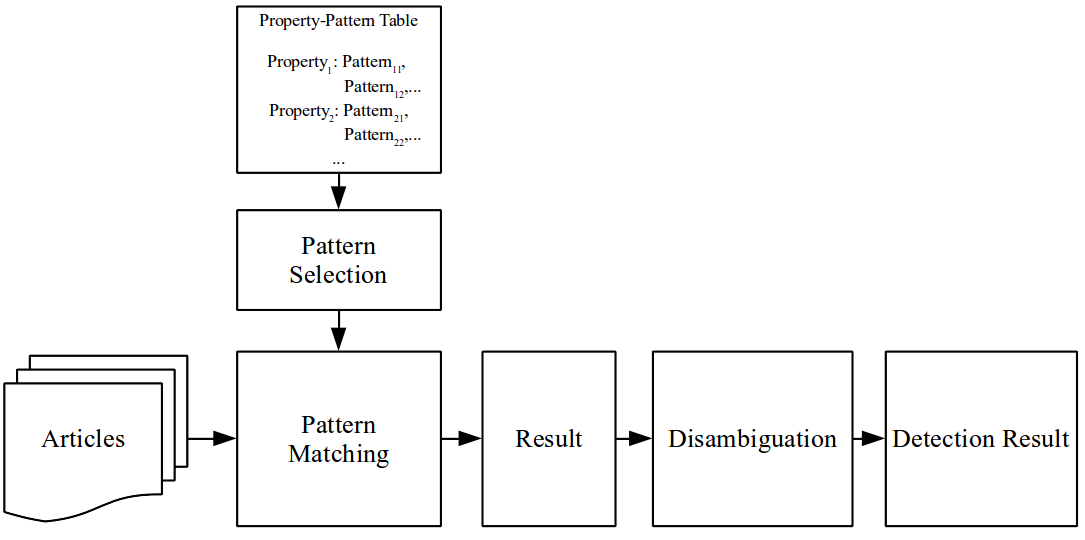
\includegraphics[width=0.9\textwidth]{images/03-process-v2}
    \caption{以樣式偵測特性流程}
    \label{i:process-v2}
\end{figure}

\begin{figure}
    \centering
    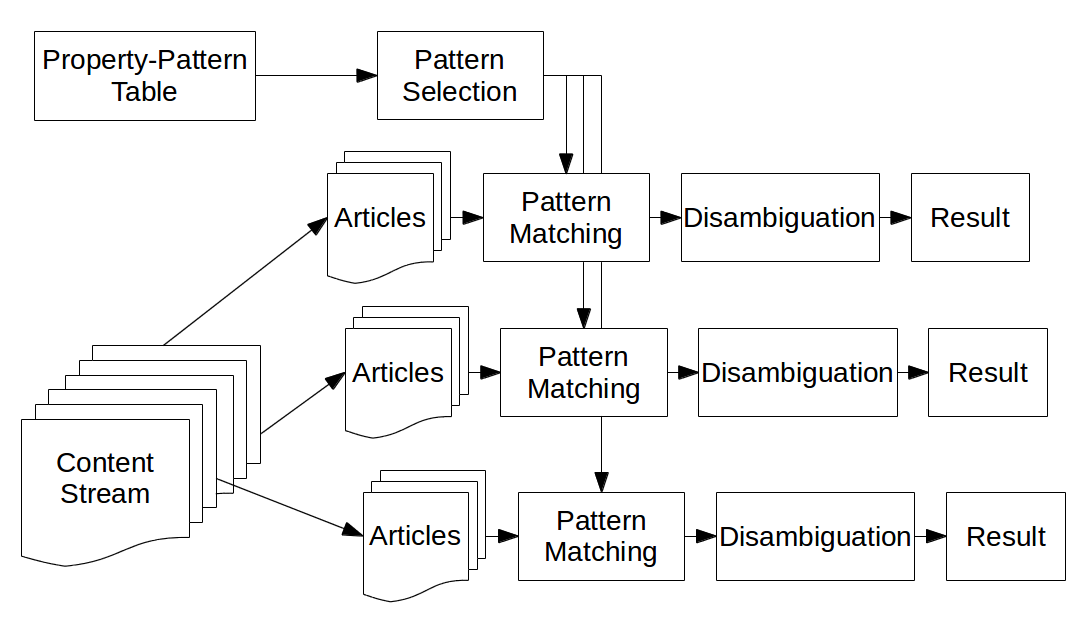
\includegraphics[width=0.9\textwidth]{images/03-pattern-parallel}
    \caption{平行處理架構}
    \label{i:process-parallel}
\end{figure}

\section{樣式比對}
\label{s:pattern-match}

樣式比對是要從句子之中確定某一個樣式是否存在,
PATTY中提供的25個YAGO關係有43,124個樣式,
但其中有不少是重複出現的,
實際上總共有19,031個獨特的樣式,
如果對每個句子都做19,031次比較顯然不是一個好方法。

為了讓樣式比對可以有效率些,
我們將所有的樣式建立成一顆前綴樹(Prefix Tree)。
先將所有首字相同的樣式合併成同一個節點,
再看第二個字是否相同,如果不同就分支出去,
依此類推,最後再連結到樣式編號,
即可透過編號查詢該樣式可能表示的實體特性。
如圖\ref{i:pattern-prefix-tree} 所示,
四個樣式「was born」、「was born at」、「was born [[det]] village」和「was bron [[det]] willage in」的首字皆為was,所以併成一個節點。
第二個字也都相同,所以也併成一個節點。
而此時「was born」已經完成了,所以born節點下新增一個樣式編號的節點。
剩下三個樣式的第三個字有詞性標記「[[det]]」和單字「at」,
便在born節點下新增[[det]]和at節點。at節點完成了「was bron at」樣式,
而[[det]]節點則繼續將後續的字加入這棵前綴樹上,
最後這棵樹上所有葉子都是一個樣式編號。

\begin{figure}
    \centering
    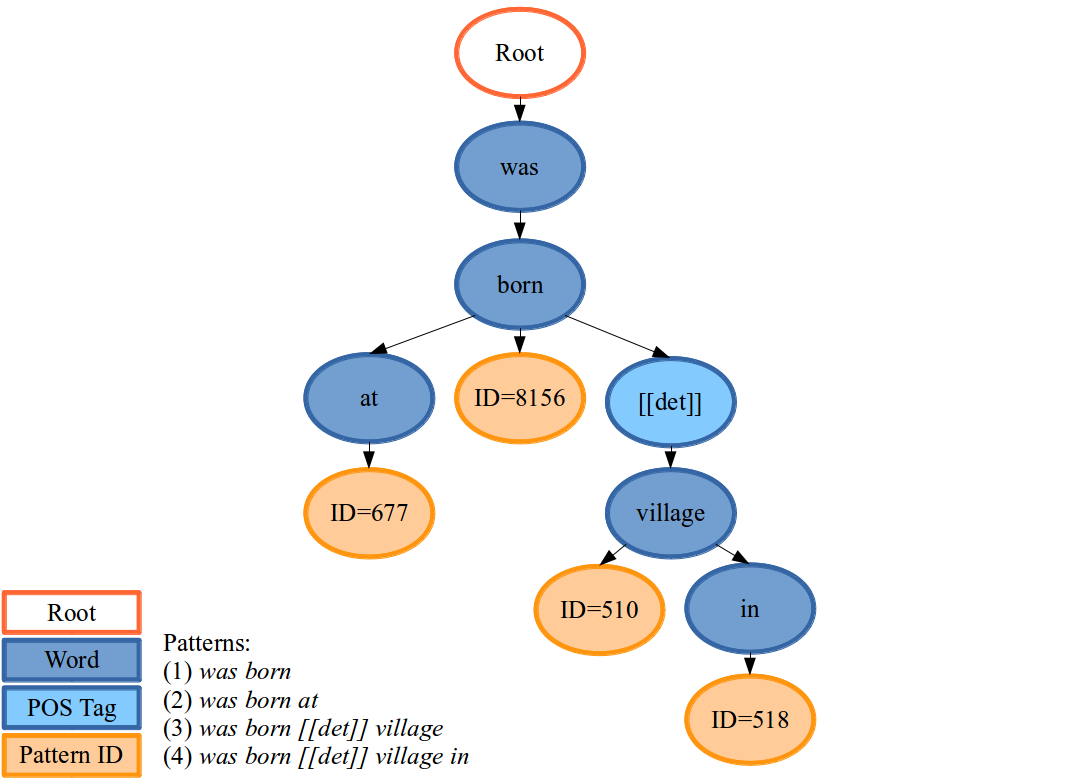
\includegraphics[width=0.9\textwidth]{images/03-pattern-prefix-tree}
    \caption{樣式前綴樹}
    \label{i:pattern-prefix-tree}
\end{figure}

有了樣式前綴樹後,
再來就是利用這棵樹來比對句子中是否有出現其中的樣式。
演算法\ref{a:pattern-match} 描述了比對的過程。

演算法\ref{a:pattern-match} 的輸入是擬比對的文章A以及已經預先建立完成的樣式前綴樹T,
輸出是文章A所出現過的樣式及其出現的位置。
對於文章A中的每個句子S,由於樣式包含詞性標記,
因此需要將S標記,實驗中使用的是Textblob的APTagger\footnote{https://github.com/sloria/textblob-aptagger}來進行快速的詞性標記。
接下來開始從句子的第一個字開始,
如果這個字或其詞性標記有出現在樣式前綴樹Root下的第一層節點中出現,
便將這個節點和此字於句子中的位置記錄下來。
再看句子中的下一個字,
此時先檢查暫存紀錄中的字是不是能夠繼續往下走這棵樣式前綴樹,
如果可以往下走代表還沒有發現樣式;
如果子節點已經是帶有樣式編號的樹葉的話,
就是發現了一個樣式,然後紀錄下來。
如果發現沒有辦法繼續往下走,
則代表在未來的步驟中不可能走到任何一個紀錄樣式編號的樹葉,
因此將這組紀錄從暫存紀錄中移除。
最後便可以知道有哪些樣式出現在文章中以及出現的位置。

\begin{algorithm}
    \caption{樣式比對演算法}
    \label{a:pattern-match}
    \begin{algorithmic}[1]
        \Require  
            $A$: 文章;
            $T$: 樣式前綴樹;
        \Ensure
            $P$: 文章$A$中出現的樣式;
        \State $P\gets$[]
        \Comment{初始化$P$}
        \ForAll{Sentence $S$ {\bf in} $A$ }
            \State 對$S$進行詞性標記
            \State $tmpP\gets$[]
            \Comment{初始化暫存陣列}
            \For{$i$ {\bf from} 0 to length of $S$}
                \State ($word$,$POStag$) $\gets$ $S[i]$
                \ForAll{$possiblePattern$ {\bf in} $tmpP$}
                    \If{$word$ or $POStag$ {\bf in} $T$'s $possiblePattern$.depthInTree+1 level nodes}
                        \State continue
                    \Else
                        \If{$T$'s $possiblePattern$.depthInTree+1 level node is $PatternID$}
                            \State {\bf add} ($PatternID$,$startPoint$,$i$ as $endPoint$) {\bf into} $P$
                        \EndIf
                        \State {\bf remove} $possiblePattern$ {\bf from} $tmpP$
                    \EndIf
                \EndFor
                \If{$word$ or $POStag$ {\bf in} $T$'s first level nodes}
                \State {\bf add} ($depthInTree$,$i$ as $startPoint$) {\bf into} $tmpP$
                \EndIf
            \EndFor
        \EndFor
        \State \Return P
    \end{algorithmic}
\end{algorithm}

演算法\ref{a:pattern-match} 中同時於暫存紀錄中的可能樣式最多只會跟樣式前綴樹的深度相同,
若文章的長度是n個字、每個字對多可能檢查暫存同前綴樹深度m次,
則演算法\ref{a:pattern-match} 的時間複雜度是O(mn)。

\section{樣式篩選}
\label{s:select-pattern}
樣式篩選是希望在建立樣式前綴樹提供樣式比對使用前,
先對樣式進行一些篩選,以解決樣式品質、可信賴度甚至是歧義問題。
針對這三個問題,主要有三種篩選的方法。

首先是關於樣式的品質,
由於PATTY對每個樣式有計算一個信心值,
例如YAGO:actedIn中的樣式「links」的信心值是0.143,
而「starred in [[det]] film」的信心值是0.937,
後者相較於前者更適合作為樣式來進行特性偵測。
這裡主要是針對信心值進行篩選,
設定信心值門檻,不使用信心值低於門檻值的樣式進行樣式比對。

再來是可信賴度的部份,
由於我們認為可信賴度是用來是樣式能不能表達特性的程度,
因此定義了計算可性度為一個樣式出現的次數中,
其出現的文件確實具有實體特性的比例。
例如,「was born」曾出現在22,543份文件之中,
其中有12,038份文件確實有「出生地」這項特性,
因此樣式「was bron」對「出生地」這項特性的可信賴度是0.534。
而「school in」曾出現在1,486份文件中,
其中有387份文件有「出生地」這項特性,其可信賴度為0.26,
相較於「was bron」來的低。
可信賴度越高代表這個樣式出現時有越高的可能可以代表存在實體特性,
反之可信賴度較低的樣式則可能根本無法掉表實體特性。
藉由可信賴度,我們可以篩選出較值得信賴的樣式進行比對。

最後是歧義的問題,有部份的樣式可能同時表示多種實體特性,
以表\ref{t:ext} 的例子來說,「lived in」同時可能表示「出生地」與「生活地」兩種實體特性,這樣的樣式我們就稱其歧義度為2,代表此樣式可以表達兩種實體特性。
表\ref{t:yago-degree} 即顯示了各信心值下各種歧義度的樣式統計,
約有40\%的樣式具有歧義,其中樣式「worked from」的歧義度甚至高達17(livesIn、
hasAcademicAdvisor、diedIn、isLeaderOf、isKnownFor、isMarriedTo、created、
influences、isLocatedIn、wasBornIn、worksAt、graduatedFrom、actedIn、produced、
directed、isCitizenOf、isPoliticianOf)。
歧義度大的樣式也可以視為沒辦法精確的表達特性,
在樣式篩選時,會將歧義度太大的樣式捨去,
避免過度混淆而影響了系統的效能。

%t:yago-degree
\begin{table}[t]
    \begin{center}
        \small
        \begin{tabular}{l||c|c|c|c}
        \hline
        歧義度 & 信心值> 0 & 信心值> 0.7 & 信心值> 0.8 & 信心值> 0.9\\
          & 樣式數量 & 樣式數量 & 樣式數量 & 樣式數量 \\
        \hline
        1 & 11381 & 8913 & 5951 & 1879 \\
        2 & 4778 & 4175 & 2328 & 316 \\
        3 & 1255 & 1048 & 683 & 187 \\
        4 & 666 & 600 & 473 & 67 \\
        5 & 635 & 605 & 278 & 18 \\
        6 & 77 & 68 & 50 & 10 \\
        7 & 132 & 131 & 52 & 12 \\
        8 & 49 & 49 & 13 & 2 \\
        9 & 26 & 26 & 12 & 8 \\
        10 & 13 & 13 & 0 & 0 \\
        11 & 12 & 12 & 9 & 5 \\
        12 & 2 & 2 & 0 & 0 \\
        13 & 0 & 0 & 0 & 0 \\
        14 & 2 & 2 & 0 & 0 \\
        15 & 0 & 0 & 0 & 0 \\
        16 & 0 & 0 & 0 & 0 \\
        17 & 3 & 3 & 0 & 0 \\
        \hline
        總計 & 19031 & 15647 & 9849 & 2504 \\
        \hline
        \end{tabular}
        \caption{樣式數量與信心值、歧異度統計}
        \label{t:yago-degree}
    \end{center}
\end{table}


\section{特性消歧義}
\label{s:pattern-disambiguity}

經過樣式篩選、比對之後,
文章中出現的樣式可以代表的特性仍可能具有歧義,
表\ref{t:yago-overlap} 就呈現了各種特性之間所屬的樣式重疊的狀況。
表中的數字代表樣式重疊的比例,沒有數字代表兩組樣式無重疊或者重疊的比例甚低。
第i排第j欄的數字是$\frac{|property\ i's\ patterns \cap property\ j's\ patterns|}{|property\ i's\ patterns|}$。
例如表中第一排第二欄的值是0.33,
代表可以用來表達actedIn的樣式之中有33\%也可以用來表達created這個特性。
表中可以看到像是diedIn、livesIn、wasBornIn互有重疊,
或是像happendIn、hasCapital、participatedIn幾乎完全不與其他特性混淆。
針對歧義問題,本研究使用了以下幾種方法嘗試消歧義。

%t:yago-overlap
\begin{table}[t]
    \begin{center}
        \scriptsize
        \begin{tabular}{l||*{12}{c}}
       & (1) & (2) & (3) & (4) & (5) & (6) & (7) & (8) & (9) & (10) & (11) & (12) \\
            \hline
            (1) actedIn  & 1.00  & 0.33  &    & 0.01  & 0.31  & 0.01  &    & 0.02  &    & 0.09  &    &   \\
            (2) created  & 0.21  & 1.00  &    & 0.01  & 0.17  & 0.11  &    & 0.01  &    & 0.10  & 0.02  & 0.03 \\
            (3) dealsWith  &    &    & 1.00  &    &    &    &    &    & 0.01  & 0.01  &    &   \\
            (4) diedIn  & 0.01  & 0.03  &    & 1.00  & 0.01  & 0.04  &    & 0.01  &    & 0.03  &    & 0.01 \\
            (5) directed  & 0.51  & 0.44  &    & 0.01  & 1.00  & 0.07  &    & 0.03  &    & 0.06  &    &   \\
            (6) graduatedFrom  & 0.01  & 0.16  &    & 0.02  & 0.04  & 1.00  &    & 0.01  &    & 0.02  &    & 0.04 \\
            (7) happenedIn  &    &    & 0.02  &    &    &    & 1.00  &    &    &    &    &   \\
            (8) hasAcademicAdvisor  & 0.06  & 0.07  &    & 0.02  & 0.06  & 0.05  &    & 1.00  &    & 0.18  &    &   \\
            (9) hasCapital  &    &    & 0.21  & 0.08  &    &    &    &    & 1.00  &    &    &   \\
            (10) hasChild  & 0.05  & 0.09  &    & 0.01  & 0.02  & 0.01  &    & 0.03  &    & 1.00  &    & 0.13 \\
            (11) hasWonPrize  & 0.08  & 0.69  &    &    & 0.01  &    &    & 0.04  &    & 0.21  & 1.00  & 0.21 \\
            (12) holdsPoliticalPosition  & 0.01  & 0.08  &    & 0.01  &    & 0.07  &    &    &    & 0.40  & 0.01  & 1.00 \\
            (13) influences  & 0.07  & 0.13  &    & 0.01  & 0.02  & 0.03  &    & 0.13  &    & 0.35  &    & 0.13 \\
            (14) isCitizenOf  & 0.02  & 0.07  &    & 0.27  & 0.02  & 0.10  &    & 0.01  &    & 0.03  &    & 0.03 \\
            (15) isKnownFor  & 0.09  & 0.48  &    & 0.04  & 0.15  & 0.24  &    & 0.10  &    & 0.18  & 0.03  & 0.05 \\
            (16) isLeaderOf  & 0.01  & 0.58  &    & 0.18  & 0.01  & 0.41  &    & 0.01  &    & 0.04  & 0.11  & 0.11 \\
            (17) isLocatedIn  &    & 0.01  & 0.02  & 0.23  &    & 0.03  &    & 0.01  &    & 0.02  &    &   \\
            (18) isMarriedTo  & 0.06  & 0.10  &    & 0.01  & 0.02  & 0.02  &    & 0.09  &    & 0.43  &    & 0.06 \\
            (19) isPoliticianOf  & 0.01  & 0.07  &    & 0.50  & 0.02  & 0.11  &    & 0.01  &    & 0.04  &    & 0.02 \\
            (20) livesIn  & 0.01  & 0.10  &    & 0.54  & 0.02  & 0.09  &    & 0.02  &    & 0.03  &    & 0.02 \\
            (21) participatedIn  & 0.02  & 0.01  &    & 0.02  & 0.01  &    &    &    &    & 0.07  &    & 0.01 \\
            (22) playsFor  &    & 0.04  &    & 0.02  &    & 0.13  &    &    &    & 0.02  &    &   \\
            (23) wasBornIn  & 0.01  & 0.03  &    & 0.55  & 0.01  & 0.06  &    & 0.02  &    & 0.02  &    &   \\
            (24) worksAt  & 0.02  & 0.35  &    & 0.04  & 0.06  & 0.63  &    & 0.02  &    & 0.03  & 0.03  & 0.06 \bigskip \\
        \end{tabular}
        \begin{tabular}{l||*{12}{c}}
                   & (13) & (14) & (15) & (16) & (17) & (18) & (19) & (20) & (21) & (22) & (23) & (24) \\
            \hline
            (1) actedIn  & 0.08  & 0.01  & 0.07  &    &    & 0.14  &    &    &    &    & 0.01  & 0.02 \\
            (2) created  & 0.10  & 0.02  & 0.23  & 0.08  &    & 0.14  & 0.01  & 0.02  &    & 0.02  & 0.01  & 0.17 \\
            (3) dealsWith  & 0.01  &    &    &    & 0.07  & 0.01  &    &    &    &    & 0.01  &   \\
            (4) diedIn  & 0.02  & 0.16  & 0.05  & 0.06  & 0.22  & 0.04  & 0.17  & 0.29  &    & 0.02  & 0.50  & 0.05 \\
            (5) directed  & 0.05  & 0.01  & 0.19  &    &    & 0.08  & 0.01  & 0.01  &    & 0.01  & 0.01  & 0.07 \\
            (6) graduatedFrom  & 0.03  & 0.04  & 0.18  & 0.09  & 0.02  & 0.05  & 0.02  & 0.03  &    & 0.09  & 0.03  & 0.47 \\
            (7) happenedIn  &    &    &    &    &    &    &    &    &    &    &    &   \\
            (8) hasAcademicAdvisor  & 0.51  & 0.01  & 0.25  &    & 0.02  & 0.59  & 0.01  & 0.02  &    &    & 0.04  & 0.05 \\
            (9) hasCapital  &    &    &    &    &    &    &    &    &    &    &    &   \\
            (10) hasChild  & 0.24  & 0.01  & 0.08  & 0.01  & 0.01  & 0.51  & 0.01  & 0.01  &    & 0.01  & 0.01  & 0.01 \\
            (11) hasWonPrize  &    & 0.04  & 0.68  & 0.64  &    &    &    & 0.04  &    &    & 0.03  & 0.64 \\
            (12) holdsPoliticalPosition  & 0.27  & 0.02  & 0.07  & 0.04  &    & 0.23  & 0.01  & 0.01  &    &    &    & 0.09 \\
            (13) influences  & 1.00  & 0.01  & 0.09  &    & 0.01  & 0.51  &    & 0.01  &    &    & 0.01  & 0.03 \\
            (14) isCitizenOf  & 0.04  & 1.00  & 0.11  & 0.22  & 0.20  & 0.07  & 0.36  & 0.39  &    & 0.06  & 0.33  & 0.13 \\
            (15) isKnownFor  & 0.14  & 0.06  & 1.00  & 0.18  & 0.03  & 0.23  & 0.04  & 0.06  &    & 0.05  & 0.05  & 0.35 \\
            (16) isLeaderOf  & 0.02  & 0.38  & 0.62  & 1.00  & 0.22  & 0.11  & 0.20  & 0.26  &    & 0.04  & 0.26  & 0.64 \\
            (17) isLocatedIn  & 0.01  & 0.12  & 0.04  & 0.08  & 1.00  & 0.03  & 0.11  & 0.17  &    & 0.01  & 0.28  & 0.03 \\
            (18) isMarriedTo  & 0.30  & 0.01  & 0.09  & 0.01  & 0.01  & 1.00  & 0.01  & 0.01  &    & 0.01  & 0.02  & 0.03 \\
            (19) isPoliticianOf  & 0.02  & 0.63  & 0.14  & 0.20  & 0.31  & 0.09  & 1.00  & 0.61  &    & 0.06  & 0.44  & 0.15 \\
            (20) livesIn  & 0.04  & 0.44  & 0.13  & 0.17  & 0.30  & 0.06  & 0.40  & 1.00  &    & 0.03  & 0.56  & 0.10 \\
            (21) participatedIn  &    &    &    &    &    & 0.07  &    &    & 1.00  &    & 0.02  & 0.02 \\
            (22) playsFor  &    & 0.03  & 0.05  & 0.01  & 0.01  & 0.01  & 0.02  & 0.02  &    & 1.00  & 0.02  & 0.11 \\
            (23) wasBornIn  & 0.03  & 0.22  & 0.07  & 0.10  & 0.30  & 0.06  & 0.17  & 0.33  &    & 0.03  & 1.00  & 0.07 \\
            (24) worksAt  & 0.04  & 0.06  & 0.34  & 0.19  & 0.03  & 0.07  & 0.04  & 0.05  &    & 0.11  & 0.05  & 1.00 \\
        \end{tabular}
        \caption{特性中樣式重疊狀態}
        \normalsize
        數字代表重疊比例,也就是有多少組樣式同時出現在其他的特性中,同時也代表了可能產生歧義的樣式比例。
        \label{t:yago-overlap}
    \end{center}
\end{table}


首先是使用實體的類型資訊。
由於PATTY的實體特性如表\ref{t:yago-relation} 有每個特性的領域(Domain)與範圍(Range),
如果可以知道被描述的實體的類型為何,就可以依據特性的領域來進行判斷。
例如特性actedIn的領域是演員(wordnet\_actor),
經過樣式比對之後有一個actedIn的樣式存在文章之中,
如樣式「appeared in」存在Wikipedia的Jahsha Bluntt條目中,
但Jahsha是籃球員(wordnet\_basketball\_player)而非演員,
如果沒有Jahsha的類型資訊,系統就會判定這篇文章存在特性actedIn,
但透過類型資訊,知道Jahsha不是演員,
就可以判斷特性actedIn不應該存在這篇文章之中。

再來對於有歧義的樣式,需要有挑選特性的策略。
當一個樣式自文章中被比對出來時,
要判斷實體特性的結果有存在一個到數個實體特性或其實沒有實體特性等可能性,
要選擇一個,多個或不選便是一個問題。
對於候選的樣式,有以下幾種選擇策略:(1) 只選一個、(2) 設定一個挑選門檻、(3) 全部都選。

這裡可以利用第\ref{s:select-pattern} 小節中提過的樣式對特性可信賴度作為選擇的依據。
在(1)只選一個的策略下,挑選候選特性中可信賴度最高的特性。
例如樣式「have lived in」的候選特性有isLocatedIn、wasBornIn、
isCitizenOf、livesIn、isLeaderOf,
在「have lived in」總共95次出現中,代表isLocatedIn有52次、wasBornIn有21次、
isCitizenOf有8次、livesIn有6次、isLeaderOf有2次,換算可信賴度分別為0.547、0.221、
0.084、0.063、0.021。
在策略(1)下,選擇可信賴度最高的isLocatedIn作為該樣式所代表的特性。
但這樣只會固定都選一個特性,沒有辦法因應可能有多個特性的情形,
因此有了策略(2),對可信賴度進行正規化,設定一個門檻以篩選之。
正規化是將所有候選特性可信賴度除以可信賴度中最大的值,
經過正規化的可信賴度分別是1、0.404、0.154、0.115、0.038。
如果門檻為0.5,那只有isLocatedIn能通過門檻。
如果門檻值設定為0.2,那麼isLocatedIn、wasBornIn都會被當作此樣式代表的特性。
透過特性選擇的策略,可以嘗試降低歧義的影響。

最後,除了使用挑選策略之外,
我們認為樣式出現的前後文對於該判定哪些實體特性存在或不存在是有影響的。
當某個描述特定的實體特性的樣式出現時可能會伴隨出現一些固定的字詞。
如果沒有那些字詞伴隨出現,有可能是與實體特性無關的句子。

例如,dealsWith是國家與國家間締約的特性,
其中樣式「divided into」若用來描述dealsWith,
前後文就常會出現一些國家名、行政區之類的詞彙等。
又例如holdsPoliticalPosition的樣式出現時,
常常會接上首相、大使、市長等詞彙。
若沒有這些詞彙伴隨的出現,常常是無關的句子。

我們希望可以利用樣式出現時,句子的前後文內的字來幫助選擇特性。
對此,
我們先從過去的文件之中把所有含有樣式的句子取出,
僅將句子中所有的字轉為小寫,並沒有其他任何處理,
將確實含有文件所屬特性的句子對該特性標上正向標記後放入該特性分類,
對於文件沒有出現的特性標上負向標記後放入特性分類。
例如文章A具有wasBornIn、isLocatedIn兩個實體特性,並有$S_1$與$S_2$兩個句子。
其中的句子$S_1$包含樣式「have lived in」,可以代表isLocatedIn、wasBornIn、
isCitizenOf、livesIn、isLeaderOf等5種特性;
句子$S_2$包含樣式「was invaded」,可以代表participatedIn、dealsWith等2種特性。
由於文章A並沒有「was invaded」可以代表的特性,
因此我們將$S_2$加上負向標記,並放入participatedIn與dealsWith的分類中。
而對$S_1$,則加上正向標記後放入wasBornIn與isLocatedIn的分類之中,
加上負向標記後放入isCitizenOf、livesIn、isLeaderOf的分類之中。
整個加上標記的流程如圖\ref{i:tagging} 所示。

\begin{figure}
    \centering
    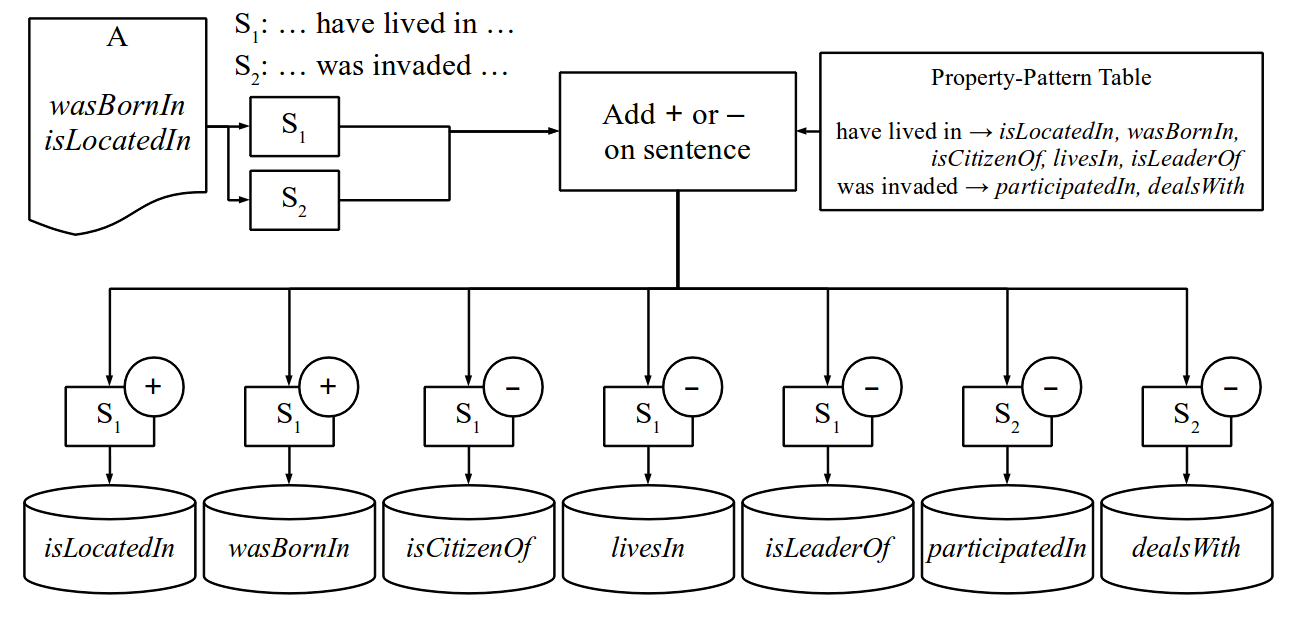
\includegraphics[width=0.9\textwidth]{images/03-tagging}
    \caption{標記句子流程}
    \label{i:tagging}
\end{figure}

每個實體特性分類中包含了許多句子,有的句子具有正向標記,
代表這個句子具有該實體特性;有的句子具有負向標記,
代表這個句子不包含該實體分類。
對於每個實體特性,我們以分類中的句子所出現過的詞作為特徵,
正、負向標記的詞頻作為特徵值,
訓練了一個二元的簡單貝氏分類器\footnote{訓練的過程與http://nlp.stanford.edu/IR-book/html/htmledition/naive-bayes-text-classification-1.html內的演算法一樣。}(Na\"{\i}ve Bayes Classifier),
用來區分是正向,也就是有包含實體特性的句子,
是負向,也就是不包含實體特性的句子。

這些分類器的使用時機是當樣式被比對出來之後,
我們知道這個樣式出現的句子以及透過樣式與特性關聯表可以查詢到候選的實體特性。
對於每個實體特性都已經有一個分類器了,
這讓每一個分類器對該句進行分類,
分類結果為正向代表句子含有該分類器所屬的特性,
反之則代表不存在該分類器所屬的實體特性。

